% !TeX document-id = {5530719d-34df-4dd8-b4b5-e6ed092c2b36}
% !TeX program = pdflatex
% !BIB program = biber
\documentclass[sigconf,natbib=false]{acmart}

% Imports Ahoy

%\usepackage[dvipsnames]{xcolor}
%\usepackage{graphicx}
\usepackage{tikz}
\usepackage{varwidth}
\usetikzlibrary{arrows.meta, calc, fit, positioning}

\usepackage{etoolbox}
\usepackage[binary-units, per-mode=symbol]{siunitx}
\robustify\bfseries
\robustify\emph
%\robustify\uline
\sisetup{detect-all, range-phrase=--, range-units=single, detect-weight=true,detect-inline-weight=math, table-format=1.3}

\makeatletter
\let\MYcaption\@makecaption
\makeatother

\usepackage[font=footnotesize]{subcaption}

\makeatletter
\let\@makecaption\MYcaption
\makeatother

%\usepackage[basic]{complexity}
\usepackage[super,negative]{nth}

\usepackage[british]{babel}
\usepackage{csquotes}

\usepackage{booktabs}
%\usepackage[
%activate={true,nocompatibility},
%final,
%tracking=true,
%kerning=true,spacing=true
%]{microtype}
%\microtypecontext{spacing=nonfrench}

\usepackage[maxnames=2,maxbibnames=99,mincrossrefs=99,sortcites,style=numeric-comp
%,backend=biber
]{biblatex}
\addbibresource{papers-off.bib}
\addbibresource{confs-off.bib}
\addbibresource{books-off.bib}
\addbibresource{rfc.bib}
\addbibresource{misc.bib}

%\DeclareFieldFormat[inproceedings]{doi}{}
%\DeclareFieldFormat[article]{doi}{}
%\DeclareFieldFormat*{url}{}
%\DeclareFieldFormat[online]{url}{\mkbibacro{URL}\addcolon\space\url{#1}}
%\DeclareFieldFormat[report]{url}{\mkbibacro{URL}\addcolon\space\url{#1}}

%picky abt et al.
\usepackage{xpatch}

\xpatchbibmacro{name:andothers}{%
	\bibstring{andothers}%
}{%
	\bibstring[\emph]{andothers}%
}{}{}

\usepackage{url}
\usepackage{hyperref}
\usepackage[nameinlink]{cleveref}
\newcommand{\crefrangeconjunction}{--}
\crefname{table}{table}{tables}

% Official colours!

\definecolor{uofguniversityblue}{rgb}{0, 0.219608, 0.396078}

\definecolor{uofgheather}{rgb}{0.356863, 0.32549, 0.490196}
\definecolor{uofgaquamarine}{rgb}{0.603922, 0.72549, 0.678431}
\definecolor{uofgslate}{rgb}{0.309804, 0.34902, 0.380392}
\definecolor{uofgrose}{rgb}{0.823529, 0.470588, 0.709804}
\definecolor{uofgmocha}{rgb}{0.709804, 0.564706, 0.47451}

\definecolor{uofglawn}{rgb}{0.517647, 0.741176, 0}
\definecolor{uofgcobalt}{rgb}{0, 0.615686, 0.92549}
\definecolor{uofgturquoise}{rgb}{0, 0.709804, 0.819608}
\definecolor{uofgsunshine}{rgb}{1.0, 0.862745, 0.211765}
\definecolor{uofgpumpkin}{rgb}{1.0, 0.72549, 0.282353}
\definecolor{uofgthistle}{rgb}{0.584314, 0.070588, 0.447059}
\definecolor{uofgpillarbox}{rgb}{0.701961, 0.047059, 0}
\definecolor{uofglavendar}{rgb}{0.356863, 0.301961, 0.580392}

\definecolor{uofgsandstone}{rgb}{0.321569, 0.278431, 0.231373}
\definecolor{uofgforest}{rgb}{0, 0.317647, 0.2}
\definecolor{uofgburgundy}{rgb}{0.490196, 0.133333, 0.223529}
\definecolor{uofgrust}{rgb}{0.603922, 0.227451, 0.023529}

% End Imports

%\usepackage[english]{babel}
\usepackage{blindtext}

% Copyright
\renewcommand\footnotetextcopyrightpermission[1]{} % removes footnote with conference info
\setcopyright{none}
%\setcopyright{acmcopyright}
%\setcopyright{acmlicensed}
%\setcopyright{rightsretained}
%\setcopyright{usgov}
%\setcopyright{usgovmixed}
%\setcopyright{cagov}
%\setcopyright{cagovmixed}

\settopmatter{printacmref=false, printccs=false, printfolios=true}

% DOI
\acmDOI{}

% ISBN
\acmISBN{}

%Conference
\acmConference[SOSR '21]{}
%\acmYear{2021}
%\copyrightyear{}

%% {} with no args suppresses printing of the price
\acmPrice{}


\begin{document}
	\title{Revisiting the Classics: Online RL in the Programmable Data-Plane}
	
	%\titlenote{Produces the permission block, and copyright information}
	%\subtitle{Extended Abstract}
	
%	\author{Paper \# XXX, XXX pages}
	 \author{Kyle A. Simpson}
	 \orcid{0000-0001-8068-9909}
	 \affiliation{%
	   \institution{University of Glasgow}
	   \city{Glasgow} 
	   \state{Scotland}
	 }
	 \email{k.simpson.1@research.gla.ac.uk}
	 \author{Dimitrios P. Pezaros}
\orcid{0000-0003-0939-378X}
	 \affiliation{%
	\institution{University of Glasgow}
	\city{Glasgow} 
	\state{Scotland}
}
\email{Dimitrios.Pezaros@gla.ac.uk}
	
	% The default list of authors is too long for headers}
	\renewcommand{\shortauthors}{Simpson \emph{et al}.}
	
\begin{abstract}
Note: below text is just the UK systems workshop abstract I submitted.	
\end{abstract}
	
\maketitle
	
\section{Introduction}

Automatic optimisation, control, and defence of networks are at last becoming commonplace. Data-driven networking has led the charge in traffic optimisation, congestion control and packet classification via adaptive techniques such as Reinforcement Learning (RL), where every change and its measured effects further improve future decisions. Considering that the network evolves in its use and deployed protocols, this flexibility is essential. Yet data-driven methods suffer from a key weakness: they are dependent on both the recency and accuracy of input state. An out-of-date view of the world will lead to suboptimal choices, as will long processing times. These can result in worse performance and slower adaptation to the evolving network.

Programmable data-planes and in-switch compute, then, hold promise for integrating these new techniques in a feasible and efficient manner (beyond dedicated servers or virtualised network functions). For RL, key tasks include policy evaluation, online training, state collection, and action execution -- each of these introduces some degree of sensitivity to state accuracy. Ideally then, all logic would run on these programmable devices. Yet, there is often a finite budget in microcode/FPGA space, per-packet processing times, and available cores for execution. Moreover, necessary hardware, such as floating-point units, is unavailable in almost all cases.

The precise costs and trade-offs which operators and designers must make have yet to be identified. This follows from a design space explosion induced by many necessary workarounds. For instance, quantisation or fixed-point arithmetic will allow training and control on all devices, but introduces further questions: what degree of quantisation is most appropriate? What effect would this have on training accuracy, communications cost, or storage requirements? More concerns arise when we consider core allocation, local vs. distributed training, and reliable lightweight communication in multi-agent scenarios. In all cases, network operators will not consider tools which affect underlying traffic.

I aim to examine the effects of these choices on an existing RL-based DDoS attack mitigation system. To protect legitimate traffic, this controls packet drop and filtering for each flow using individual metrics observed by RL agents at ingress routers, and load measurements from several points along the path taken by the flow in question. The examined metrics include the throughput and latency of its individual components alongside system metrics: flow arrival-to-judgement time, and knowledge propagation time. Beyond this, it's crucial to identify what we can implement on pure P4-capable hardware. While extensions to P4 are fairly common in commodity hardware, the need for full design access (as in NetFPGA) or Micro-C (as in Netronome SmartNICs) represent a break from the clean, loop-free semantics of P4. As the market matures, these may represent different feature classes and price points.

I will discuss early development efforts (including challenges and results) on the Netronome Agilio SmartNIC, which supports the P4 language as well as some degree of arbitrary microcode. I intend to present how reinforcement learning execution and network telemetry will differ in the above metrics when compared to a vNF-based deployment (i.e., software on external commodity servers).

\section{Motivation}

\begin{figure}
	\begin{subfigure}{0.45\linewidth}
		\resizebox{\linewidth}{!}{
			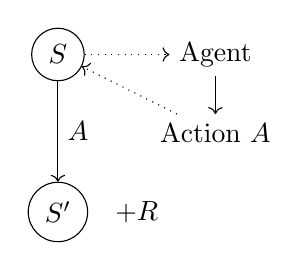
\begin{tikzpicture}
					\node[circle, draw] (state) {$S$};
					\node[circle, draw] (state') at ($(state) + (0, -2)$) {$S'$};
					
					\node (agent) at ($(2, 0) + (state)$) {Agent};
					\node[below of=agent] (action) {Action $A$};
					
					\node[right of=state'] {$+ R$};
					
					\draw[->] (state) -- (state') node[midway, right] {$A$};
					
					\draw[dotted, ->, bend left = 30] (state) -- (agent);
					\draw[->] (agent) -- (action);
					\draw[dotted, ->] (action) -- (state);
		\end{tikzpicture}}
		\caption{Theory: state measurement, action computation, and learning are zero-cost.}
	\end{subfigure}
	\begin{subfigure}{0.45\linewidth}
		\resizebox{\linewidth}{!}{
			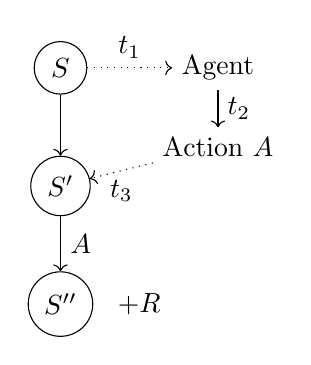
\begin{tikzpicture}
					\node[circle, draw] (state) {$S$};
					\node[circle, draw] (state') at ($(state) + (0, -1.5)$) {$S'$};
					\node[circle, draw] (state'') at ($(state') + (0, -1.5)$) {$S''$};
					
					\node (agent) at ($(2, 0) + (state)$) {Agent};
					\node[below of=agent] (action) {Action $A$};
					
					\node[right of=state''] {$+ R$};
					
					\draw[->] (state) -- (state') node[midway, right] {$\varnothing$};
					\draw[->] (state') -- (state'') node[midway, right] {$A$};
					
					\draw[dotted, ->, bend left = 30] (state) -- (agent) node[midway, above] {$t_1$};
					\draw[->] (agent) -- (action) node[midway, right] {$t_2$};
					\draw[dotted, ->] (action) -- (state') node[midway, below] {$t_3$};
		\end{tikzpicture}}
		\caption{Reality: costs of measurement and action lead to \emph{state drift}---over a time delay $t_1+t_2+t_3$, inaction transforms state $S$ into $S'$.}
	\end{subfigure}
\caption{Asynchronous RL delays and state slippage (policy updates omitted).\label{fig:state-slip}}
\end{figure}

What is our goal?

\begin{itemize}
	\item Research into asynchronous RL shows that clever reordering and mitigation can reduce the effects of state slippage on learning time and on accuracy of actions. However, it cannot completely eliminate the effect of state evolving due to the costs of action computation, execution, and policy updates~\cite{DBLP:journals/firai/TravnikMSP18}.
	\begin{itemize}
		\item What can I do with these observations?
		\begin{itemize}
			\item Reordering steps in an actively learning system is a necessary part in reducing state-slippage on learning.
			\item Minimising these effects needs us to build our system explicitly to reduce this further.
		\end{itemize}
		\item What can I do to address this?
		\begin{itemize}
			\item Reduce the time required to compute an action, to react to state, and to install that action in the network.
			\item Ensure that state is measured at agent (on-chip, or close by).
			\item Ensure actions are computed as close to where they occur as possible.
		\end{itemize}
		\item How are these being addressed?
		\begin{itemize}
			\item Place agents/decision-making as close to the switch as possible.
		\end{itemize}
		\item What applications is this affecting?
		\begin{itemize}
			\item Time-sensitive RL: DDoS mitigation, Congestion-control algorithms, ...
		\end{itemize}
		\item What would its solution be useful for?
		\begin{itemize}
			\item Make actions taken more ``correct'' (as underlying state change has been reduced).
			\item In online settings, reduce the noise of the state-action-reward function being learned.
		\end{itemize}
	\end{itemize}
	
	\item What if we do stop the world (i.e., block operation) to ensure this doesn't happen? In case of congestion control, significant throughput drops (as DNN inference takes \SI{30}{\milli\second}), so asynchrony is necessary~\cite{DBLP:journals/corr/abs-1910-04054}.
	\begin{itemize}
		\item What can I do with these observations?
		\begin{itemize}
			\item We can't pause operation of a system to collect more state, while updating the model, or while choosing an action.
		\end{itemize}
		\item What can I do to address this?
		\begin{itemize}
			\item Use state coalescing measures like in \textcite{DBLP:journals/tnsm/SimpsonRP20} and \textcite{DBLP:journals/corr/abs-1910-04054}.
		\end{itemize}
		\item What applications is this affecting?
		\begin{itemize}
			\item Congestion control algorithms primarily, others where some system depends on the output of an RL agent.
		\end{itemize}
	\end{itemize}
	
	\item Training deep RL models has its own costs (need many parallel simulations). What if we only have one stream of experience to learn from? E.g., evolution of the system is too difficult to predict and model. In general, DNNs can't be trained effectively from a single, online, real-time stream of experience.
	\begin{itemize}
		\item What can I do with these observations?
		\begin{itemize}
			\item This suggests that we should also look into non-DNN based RL approaches, if we find that RL is the best tool for the job.
		\end{itemize}
		\item What can I do to address this?
		\begin{itemize}
			\item Employ classical RL methods, which don't need many streams of parallel execution traces to learn effectively.
		\end{itemize}
		\item If addressed, what do I use them for?
		\begin{itemize}
			\item There's ongoing research which attempts to execute NN/DNN-based RL/ML models in switches, but these work under heavy concessions. Need binarisation, reduced accuracy, can't run backpropagation on SmartNIC hardware...
			\item Training and format conversion must happen off of the device, so can't be done online.
		\end{itemize}
		\item What applications is this affecting?
		\begin{itemize}
			\item In-network RL applications needing real-time evolution, where DNN online training is not doable.
			\item Likely invites some accuracy impact---linear (e.g., tile-coded) function approximation not as expressive or powerful as DNNs.
		\end{itemize}
		\item What would its solution be useful for?
		\begin{itemize}
			\item Ensures that online learning is possible in the contexts we're interested in.
			\item I.e., DDoS prevention (evolving problem).
		\end{itemize}
	\end{itemize}
	
	\item PDP hardware is advertised as supporting P4, EBPF... But almost all implementations compile to a more complex/expressive language. Presence of externs is almost universal when it comes to in-switch compute---i.e., Tofino Native Architecture\footnote{\url{    https://www.barefootnetworks.com/products/brief-p4-studio/}}, Netronome Micro-C\footnote{\url{https://www.netronome.com/products/datapath-programming-tools/}}, P4$\rightarrow$NetFPGA toolchain\footnote{\url{https://github.com/NetFPGA/P4-NetFPGA-public}}.
	\begin{itemize}
		\item What can I do with these observations?
		\begin{itemize}
			\item We should use P4 where possible to make implementation of in-network compute possible.
			\item \emph{But} we would be remiss not to make use of the multicore, general-purpose compute that many of these devices are fundamentally built to do.
			\item In-network compute and/or PDPs give us the tools we need to put RL action computation, the mechanism of action, and state measurement at the same location in the network!
		\end{itemize}
		\item If addressed, what do I use them for?
		\begin{itemize}
			\item Identify the common aspects of non-NetFPGA P4-capable devices.
			\item Determine whether these allow a common architecture (but not common reimplementation since different languages, low-level specifics).
			\item Might need to describe the same mechanism as implemented in both Netronome and Barefoot?
		\end{itemize}
		\item What applications is this affecting?
		\begin{itemize}
			\item PDP applications in general.
		\end{itemize}
	\end{itemize}
\end{itemize}

What aspects of the state-of-the-art are relevant here?

\begin{itemize}
	\item Hmmm...
\end{itemize}

\section{Techniques}

What does the hardware give us, and what can we assume are present on many other classes of device?
\begin{itemize}
	\item 96-core (\emph{management engine}, ME) (? check), grouped into \emph{islands} based on local capabilities. Fast transfer between MEs on same island (\emph{nearest neighbour registers}, NNRs)
	
	\begin{itemize}
		\item Multicore model common.
		\item Arch-specific: one program per ME. Enables cooperative scheduling between \numrange{4}{8} threads, zero-cost context switch due to register file (below).
	\end{itemize}

	\item Explicit memory hierarchy:
	
	\begin{itemize}
		\item Large register file split disjointly between threads. (likely common)
		\item Transparent cache.
		\item In order of speed? Reg file, External Mem
	\end{itemize}

	\item One program to a core---enables cooperative scheduling with zero-cost context switches.
	
\end{itemize}
Now how do we make this work?
\begin{itemize}
	\item No floating point math. Solution? Quantisation (cite some other papers who've used this to decent effect).
	
	\item Bump-in-the-wire design for SmartNIC.
	
	\item P4 for easy packet parsing, control packet extraction, passthrough and manipulation of other traffic.
	
	\item RL Island keeps freelist, P4 PIF Islands copy packets over (could in theory hack P4 firmware micro-C libraries to stop freeing resources and just pass those?).
	
	\item Control packets marked by custom \emph{experimenter} DSCP (as in \textcite{DBLP:conf/isca/LiLYCSH19}). Infrastructure can ensure that only trusted internal nodes can produce such packets.
	
	\item Control allows adaptation to any policy design assuming standard tile-coding, for any target application. Policies may be installed via block copy, or trained online. (So long as policy meets compiled maximum dimensions, constraints.)
	
	\item (not impl'd yet) How does state work? Packet passed in over work queue to control ME. source can be either the network (same mechanism as control packets)
	
	\item (not impl'd yet) How do actions work? 2 options.
	\begin{enumerate}
		\item Produce packet on wire according to config (custom format).
		\item Pass packet to local island/ME (requires both config and custom build).
	\end{enumerate}

	\item Built with \Textcite{DBLP:journals/tnsm/SimpsonRP20} in mind, but applicable to any RL application.
	
	\item New PDPs have encryption primitives: scope to include authentication etc. around control packets.
	
	\item (Not impl'd yet) Event loop can easily run on Control ME: timing APIs exposed to generate periodic events in lieu of something like \textcite{DBLP:conf/hotnets/IbanezABM19}.
\end{itemize}

\begin{figure}
	\centering
	\resizebox{\linewidth}{!}{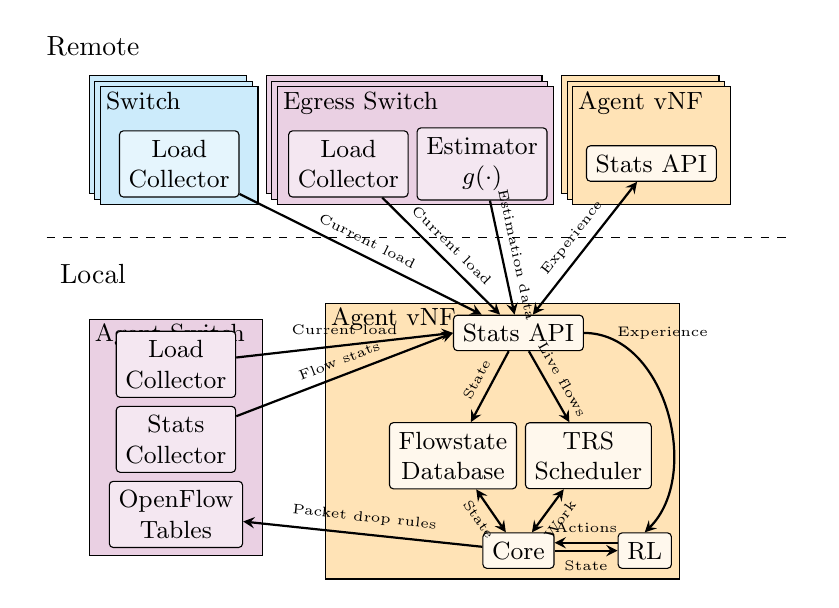
\begin{tikzpicture}
		\node(remote){Remote};
		
		%%%
		
		\node[below=0.05 of remote](swpos){};
		\node[fill=white!80!uofgcobalt, draw=black, minimum height=1.5cm, minimum width=2cm, below right= 0.1 of swpos.north west](sw1){};
		\node[fill=white!80!uofgcobalt, draw=black, minimum height=1.5cm, minimum width=2cm, below right= 0.1 of sw1.north west](sw2){};
		\node[fill=white!80!uofgcobalt, draw=black, minimum height=1.5cm, minimum width=2cm, below right= 0.1 of sw2.north west](switch){};
		\node[below right, inner sep=2pt] at (switch.north west) {\small Switch};
		\node[fill=white!90!uofgcobalt, draw, rectangle, rounded corners=0.05cm, above=0.1] (oswlc) at (switch.south) {\begin{varwidth}{1.5 cm}\small \centering Load\\Collector\end{varwidth}};
		
		%
		
		\node[right=2 of swpos](epos){};
		\node[fill=white!80!uofgthistle, draw=black, minimum height=1.5cm, minimum width=3.5cm, below right= 0.1 of epos.north west](e1){};
		\node[fill=white!80!uofgthistle, draw=black, minimum height=1.5cm, minimum width=3.5cm, below right= 0.1 of e1.north west](e2){};
		\node[fill=white!80!uofgthistle, draw=black, minimum height=1.5cm, minimum width=3.5cm, below right= 0.1 of e2.north west](egress){};
		\node[below right, inner sep=2pt] at (egress.north west) {\small Egress Switch};
		\node[fill=white!90!uofgthistle, draw, rectangle, rounded corners=0.05cm, above=0.1] (eglc) at ($(egress.south) + (-0.85,0)$) {\begin{varwidth}{1.5 cm}\small \centering Load\\Collector\end{varwidth}};
		\node[fill=white!90!uofgthistle, draw, rectangle, rounded corners=0.05cm, right=0.1] (egest) at (eglc.east) {\begin{varwidth}{1.5 cm}\small \centering Estimator\\$g(\cdot)$\end{varwidth}};
		
		%
		
		\node[right=3.5 of epos](apos){};
		\node[fill=white!60!uofgpumpkin, draw=black, minimum height=1.5cm, minimum width=2cm, below right= 0.1 of apos.north west](a1){};
		\node[fill=white!60!uofgpumpkin, draw=black, minimum height=1.5cm, minimum width=2cm, below right= 0.1 of a1.north west](a2){};
		\node[fill=white!60!uofgpumpkin, draw=black, minimum height=1.5cm, minimum width=2cm, below right= 0.1 of a2.north west](otheragent){};
		\node[below right, inner sep=2pt] at (otheragent.north west) {\small Agent vNF};
		\node[fill=white!90!uofgpumpkin, draw, rectangle, rounded corners=0.05cm, above=0.3] (oasa) at (otheragent.south) {\begin{varwidth}{1.5 cm}\small \centering Stats API\end{varwidth}};
		
		%
		
		\node[below=2.3 of remote.west](linestart){};
		\path let \p1 = (linestart) in node (lineend) at (9,\y1){};
		\draw [dashed] (linestart) -- (lineend);
		
		%%%
		
		\node[below=2.4 of remote](local){Local};
		
		%%%
		
		\node[below=0.25 of local](aswpos){};
		\node[fill=white!80!uofgthistle, draw=black, minimum height=3cm, minimum width=2.2cm, below right= 0.1 of aswpos.north west](aswitch){};
		\node[below right, inner sep=2pt] at (aswitch.north west) {\small Agent Switch};
		\node[fill=white!90!uofgthistle, draw, rectangle, rounded corners=0.05cm, above=0.1] (aswoft) at (aswitch.south) {\begin{varwidth}{1.5 cm}\small \centering OpenFlow\\Tables\end{varwidth}};
		\node[fill=white!90!uofgthistle, draw, rectangle, rounded corners=0.05cm, above=0.1] (aswsc) at (aswoft.north) {\begin{varwidth}{1.5 cm}\small \centering Stats\\Collector\end{varwidth}};
		\node[fill=white!90!uofgthistle, draw, rectangle, rounded corners=0.05cm, above=0.1] (aswlc) at (aswsc.north) {\begin{varwidth}{1.5 cm}\small \centering Load\\Collector\end{varwidth}};
		
		%
		
		\node (avfpos) at ($(aswpos) + (3,0.2)$){};
		\node[fill=white!60!uofgpumpkin, draw=black, minimum height=3.5cm, minimum width=4.5cm, below right= 0.1 of avfpos.north west](avf){};
		\node[below right, inner sep=2pt] at (avf.north west) {\small Agent vNF};
		\node[fill=white!90!uofgpumpkin, draw, rectangle, rounded corners=0.05cm, below=0.15] (avfsa) at ($(avf.north) + (0.2,0)$) {\begin{varwidth}{1.5 cm}\small \centering Stats API\end{varwidth}};
		\node[fill=white!90!uofgpumpkin, draw, rectangle, rounded corners=0.05cm, below=0.9] (avfdb) at (avfsa.south west) {\begin{varwidth}{1.5 cm}\small \centering Flowstate\\Database\end{varwidth}};
		\node[fill=white!90!uofgpumpkin, draw, rectangle, rounded corners=0.05cm, right=0.1] (avfsched) at (avfdb.east) {\begin{varwidth}{1.5 cm}\small \centering TRS\\Scheduler\end{varwidth}};
		\node[fill=white!90!uofgpumpkin, draw, rectangle, rounded corners=0.05cm, below=2.3] (avfcore) at (avfsa.south) {\begin{varwidth}{1.5 cm}\small \centering Core\end{varwidth}};
		\node[fill=white!90!uofgpumpkin, draw, rectangle, rounded corners=0.05cm, right=0.8] (avfrl) at (avfcore.east) {\begin{varwidth}{1.5 cm}\small \centering RL\end{varwidth}};
		
		%%%
		
		\tikzset{>=stealth}
		
		\draw[thick, ->] (aswlc) -- (avfsa.west) node[midway,above] {\tiny Current load};
		\draw[thick, ->] (aswsc) -- (avfsa.west) node[midway,sloped, above] {\tiny Flow stats};
		
		\draw[thick, ->] (oswlc) -- (avfsa) node[midway,above, sloped] {\tiny Current load};
		
		\draw[thick, ->] (eglc) -- (avfsa) node[midway,above, sloped] {\tiny Current load};
		\draw[thick, ->] (egest) -- (avfsa) node[midway,above, sloped] {\tiny Estimation data};
		
		\draw[thick, <->] (oasa) -- (avfsa) node[midway,above, sloped] {\tiny Experience};
		
		\draw[thick, ->] (avfsa) -- (avfdb) node[midway,above, sloped] {\tiny State};
		\draw[thick, ->] (avfsa) -- (avfsched) node[midway,above, sloped] {\tiny Live flows};
		
		\draw[thick, ->] (avfcore) -- (aswoft) node[midway,above, sloped] {\tiny Packet drop rules};
		\draw[thick, <->] (avfcore) -- (avfdb) node[midway,below, sloped] {\tiny State};
		\draw[thick, <->] (avfcore) -- (avfsched) node[midway,below, sloped] {\tiny Work};
		\draw[thick, <-] ($(avfcore.east) + (0,0.1)$) -- ($(avfrl.west) + (0,0.1)$) node[midway,above, sloped] {\tiny Actions};
		\draw[thick, ->] (avfcore) -- (avfrl) node[midway,below, sloped] {\tiny State};
		
		\draw[thick, ->] (avfsa.east) to [out=0, in=45] (avfrl.north);
		\node[right=0.3] at (avfsa.east) {\tiny Experience};
		\end{tikzpicture}}
	\caption{
		System architecture  for our RL-driven DDoS defence system.
		\label{fig:sys-arch}
	}
\end{figure}

\begin{figure}
	\centering
	\resizebox{1.2\linewidth}{!}{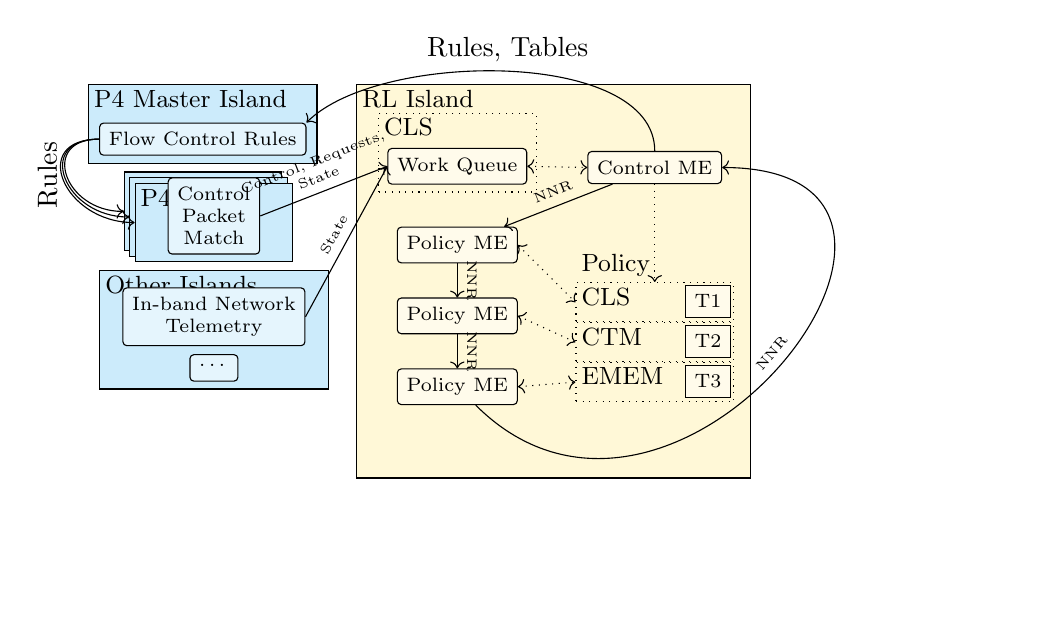
\begin{tikzpicture}
		\node[fill=white!80!uofgcobalt, draw=black, minimum height=1cm, minimum width=2.9cm](p4-master){};
		\node[below right, inner sep=2pt] at (p4-master.north west) {\small P4 Master Island};
		\node[fill=white!90!uofgcobalt, draw, rectangle, rounded corners=0.05cm, above=0.1] (p4-rules) at (p4-master.south) {\begin{varwidth}{2.5 cm}\scriptsize \centering Flow Control Rules\end{varwidth}};
		
		\node[fill=white!80!uofgcobalt, draw=black, minimum height=1cm, minimum width=2cm, below = 0.1 of p4-master](sw1){};
		\node[fill=white!80!uofgcobalt, draw=black, minimum height=1cm, minimum width=2cm, below right= 0.1 of sw1.north west](sw2){};
		\node[fill=white!80!uofgcobalt, draw=black, minimum height=1cm, minimum width=2cm, below right= 0.1 of sw2.north west](switch){};
		\node[below right, inner sep=2pt] at (switch.north west) {\small P4 Island};
		\node[fill=white!90!uofgcobalt, draw, rectangle, rounded corners=0.05cm, above=0.1] (oswlc) at (switch.south) {\begin{varwidth}{1.5 cm}\scriptsize \centering Control Packet Match\end{varwidth}};
		
		\node[fill=white!80!uofgcobalt, draw=black, minimum height=1.5cm, minimum width=2.9cm, below= 0.1 of switch](others){};
		\node[below right, inner sep=2pt] at (others.north west) {\small Other Islands};
		\node[fill=white!90!uofgcobalt, draw, rectangle, rounded corners=0.05cm, above=0.1] (others-etc) at (others.south) {\begin{varwidth}{2.5 cm}\scriptsize \centering \textellipsis \end{varwidth}};
		\node[fill=white!90!uofgcobalt, draw, rectangle, rounded corners=0.05cm, above=0.1] (others-int) at (others-etc.north) {\begin{varwidth}{2.5 cm}\scriptsize \centering In-band Network Telemetry\end{varwidth}};
		
		\node[fill=white!80!uofgsunshine, draw=black, minimum height=5cm, minimum width=5cm](rli) at ($(p4-master.east) + (3, -2)$){};
		\node[below right, inner sep=2pt] at (rli.north west) (rli-text) {\small RL Island};
		
		\node[draw=black, dotted, minimum height=1cm, minimum width=2cm](wq-out) at ($(rli-text.south) + (0.5,-0.5)$){};
		\node[below right, inner sep=2pt] at (wq-out.north west) {\small CLS};
		\node[fill=white!90!uofgsunshine, draw, rectangle, rounded corners=0.05cm, above=0.1] (wq-in) at (wq-out.south) {\begin{varwidth}{2.5 cm}\scriptsize \centering Work Queue\end{varwidth}};
		
		\node[fill=white!90!uofgsunshine, draw, rectangle, rounded corners=0.05cm, above=0.1] (loop) at ($(wq-out.east) + (1.5,-0.5)$) {\begin{varwidth}{2.5 cm}\scriptsize \centering Control ME\end{varwidth}};
		
		\node[draw=black, dotted, minimum height=0.5cm, minimum width=2cm](policy-cls-out) at ($(loop.south) + (0,-1.5)$){};
		\node[below right, inner sep=2pt] at (policy-cls-out.north west) {\small CLS};
		\node[above right, inner sep=2pt] at (policy-cls-out.north west) {\small Policy};
		\node[draw=black, dotted, minimum height=0.5cm, minimum width=2cm](policy-ctm-out) at ($(policy-cls-out.south) + (0,-0.25)$){};
		\node[below right, inner sep=2pt] at (policy-ctm-out.north west) {\small CTM};
		\node[draw=black, dotted, minimum height=0.5cm, minimum width=2cm](policy-emem-out) at ($(policy-ctm-out.south) + (0,-0.25)$){};
		\node[below right, inner sep=2pt] at (policy-emem-out.north west) {\small EMEM};
		
		\node[fill=white!90!uofgsunshine, draw, rectangle, above=0.1, below left= 0.05] (t1) at (policy-cls-out.north east) {\begin{varwidth}{2.5 cm}\scriptsize \centering T1\end{varwidth}};
		\node[fill=white!90!uofgsunshine, draw, rectangle, above=0.1, below left= 0.05] (t2) at (policy-ctm-out.north east) {\begin{varwidth}{2.5 cm}\scriptsize \centering T2\end{varwidth}};
		\node[fill=white!90!uofgsunshine, draw, rectangle, above=0.1, below left= 0.05] (t3) at (policy-emem-out.north east) {\begin{varwidth}{2.5 cm}\scriptsize \centering T3\end{varwidth}};
		
		\node[fill=white!90!uofgsunshine, draw, rectangle, rounded corners=0.05cm, above=0.1] (po-me-1) at ($(wq-out.south) + (0,-1.0)$) {\begin{varwidth}{2.5 cm}\scriptsize \centering Policy ME\end{varwidth}};
		
		\node[fill=white!90!uofgsunshine, draw, rectangle, rounded corners=0.05cm, above=0.1] (po-me-2) at ($(po-me-1.south) + (0,-1.0)$) {\begin{varwidth}{2.5 cm}\scriptsize \centering Policy ME\end{varwidth}};
		
		\node[fill=white!90!uofgsunshine, draw, rectangle, rounded corners=0.05cm, above=0.1] (po-me-3) at ($(po-me-2.south) + (0,-1.0)$) {\begin{varwidth}{2.5 cm}\scriptsize \centering Policy ME\end{varwidth}};
		
		\draw[->] (loop.north) [out=90,in=45,looseness=0.75] to node[pos=0.5, rotate=0, anchor=center, above] {Rules, Tables}(p4-rules.north east);
		
		\draw[->] (p4-rules.west)  to [out=180,in=180,looseness=2]  node[pos=0.5, rotate=90, anchor=center, above] {Rules}(sw1);
		\draw[->] (p4-rules.west)  to [out=180,in=180,looseness=2] (sw2);
		\draw[->] (p4-rules.west)  to [out=180,in=180,looseness=2] (switch);
		
		\draw[->] (oswlc.east)  to node[midway, above, sloped] {\begin{varwidth}{2.5cm}\tiny \centering Control, Requests,\\State\end{varwidth}} (wq-in.west);
		\draw[->] (others-int.east)  to node[midway, above, sloped] {\tiny State} (wq-in.west);
		\draw[<->, dotted] (wq-in.east)  to (loop.west);
		\draw[->, dotted] (loop.south) to (policy-cls-out);
		
		\draw[<->, dotted] (po-me-1.east) to (policy-cls-out.west);
		\draw[<->, dotted] (po-me-2.east) to (policy-ctm-out.west);
		\draw[<->, dotted] (po-me-3.east) to (policy-emem-out.west);
		
		\draw[->] (loop) to node[midway, above, sloped] {\tiny NNR} (po-me-1);
		\draw[->] (po-me-1) to node[midway, above, sloped] {\tiny NNR} (po-me-2);
		\draw[->] (po-me-2) to node[midway, above, sloped] {\tiny NNR} (po-me-3);
		\draw[->] (po-me-3) to [out=-45,in=0,looseness=2.15] node[midway, above, sloped] {\tiny NNR} (loop);
		\end{tikzpicture}}
	\caption{Architecture for generalised RL agent on Netronome hardware.\label{fig:netro-arch}}
\end{figure}

\section{Evaluation}

How do we evaluate this without looking into classification performance?
\begin{itemize}
	\item Analytically?
	\begin{enumerate}
		\item Prove that tile splitting scheme over memory hierarchy can improve performance.
		\begin{itemize}
			\item Hit rate of different tiles according to tile dimensionality?
			\item Access time for each tier of memory hierarchy.
		\end{itemize}
	\end{enumerate}
	\item Experimentally?
	\begin{enumerate}
		\item Create ``VNF'' testbed: mirror traffic from switch to a host for telemetry processing/flow state. Send flow state over to another node who computes RL actions. RL actions installed on switch.
		\begin{itemize}
			\item Why not co-host RL computation with telemetry? Could be separate functions, could want to ensure that neither impacts the performance of the other.
		\end{itemize}
		\item Create ``PDP'' testbed: Load firmware, pass in traffic. Traffic processing/action compute/table mod occurs in PDP.
		\item What traffic? Healthy mix of attack (UDP), Discord legit Opus VoIP traffic, HTTP bulk-transfer traffic.
		\item Measure $t_{1 \cdots 3}$ according to \cref{fig:state-slip} in both VNF and PDP contexts.
		\begin{description}
			\item[$t_1$]
			\begin{description}
				\item[PDP] Packet ingress $\rightarrow$ INT Island $\rightarrow$ State arrival in Control ME.
				\item[VNF] Packet mirror time $\rightarrow$ telemetry VNF $\rightarrow$ state arrival in agent vnf.
			\end{description}
		
			\item[$t_2$]
			\begin{description}
				\item[PDP] Time to compute action over parallel Policy MEs (RL Island, SmartNIC).
				\item[VNF] Time to compute action in host program (on VNF) from received state.
			\end{description}
		
			\item[$t_3$]
			\begin{description}
				\item[PDP] Modify local tables across ME/Island boundaries (same device), verify rule present (or get ACK).
				\item[VNF] Generate OpenFlow control messages, send OF message to switch, verify rule present (or get ACK).
			\end{description}
		\end{description}
		\item HYPOTHESIS: PDP will present a reduction in these three times for per-flow state.
		\item QUESTION: Does same apply to learning?
		\item NOTE: since we're not actually assessing the \emph{quality} of output decisions, we can cut corners on what data is sent out and where. I.e., in-band network telemetry island can be skipped, if we move over representative volumes of state to/from the RL island with approximately correct delay as recorded by other studies.
	\end{enumerate}
\end{itemize}
I can think of one way to evaluate this if we employ classification performance:
\begin{enumerate}
	\item Run the existing work~\cite{DBLP:journals/tnsm/SimpsonRP20}, acquire a policy for one node after full info sharing.
	\item Load this policy onto the RL Island (\cref{fig:netro-arch}).
	\item Either feed in raw state packets, or feed in traffic if we can get INT working.
	\item For each level of quantisation needed, examine average performance.
	\item Don't compare against old numbers for final perf: use a ``VNF'' setup similar to above---this will probably suffer a bit compared to old results, where everything was on the same machine. Make it relative/normalised.
\end{enumerate}

\section{Bullets on (intended) design.}
See also: \cref{fig:netro-arch}.
\begin{itemize}
	\item High-level overview.
	\begin{itemize}
		\item RL operations \emph{do not happen on the core path}.
		\item Another island (or set of cores) is dedicated to handling inputs, configuration, computation.
		\item Cross-island communication happens over \emph{rings} (Netronome-specific).
		\begin{itemize}
			\item E.g., this is how the P4 firmware propagates rules from master island to P4 workers.
			\item My impl.\ specific---shared freelist for memory pointers in EMEM.
		\end{itemize}
		\item Controller is \emph{always} co-hosted, interfaces over PCI-e. This also applies to Barefoot Tofino.
	\end{itemize}
	\item Policy configuration.
	\begin{itemize}
		\item (Re)-configurable at runtime.
		\item Custom DSCP marker acts as indicator of RL packets (i.e., bother with parsing past UDP).
		\item P4 parser extracts headers, parser state and payload passed over ring to another core dedicated to RL operations.
		\item Policy dimensions, size, action count, tiling strategies, learning parameters ($\alpha, \gamma, \epsilon$, related falloffs) can all be chosen and changed live.
	\end{itemize}
	\item State Handling.
	\begin{itemize}
		\item State input to model \emph{always} should produce an action.
		\item State vectors should come from elsewhere on the device: this may either be a dedicated island/core cluster (i.e., also performing INT management), or it may be a packet from the network.
	\end{itemize}
	\item Action Handling.
	\begin{itemize}
		\item A state vector is tile coded, action probabilities are produced, and an action is chosen according to current choice of $\epsilon$ (exploration parameter).
		\item \emph{Open question: how to configure action destination? This should either be another core (after an optional transformation), a packet sent out to a destination, maybe talk back to the controller.}
	\end{itemize}
	\item Learning.
	\begin{itemize}
		\item \emph{Open question: how to safely \& reasonably map state back to incoming rewards?}
		\item \emph{Open question: Can/should this also support on-chip reward signals?}
	\end{itemize}
\end{itemize}

\section{What's implemented 'til now?}
System?
\begin{itemize}
	\item Core-to-core communication.
	\item P4 parser for relevant packets.
	\item Packet copy + handoff from P4 to RL MEs.
	\item Dynamic base configuration.
	\item Dynamic tiling configuration.
	\item Policy installation via block-copy.
	\item Packet generation for above config functions, as well as policy quantisation and splitting.
	\item Tile-coding of quantised states on-chip, and state packet receipt.
\end{itemize}

Experiments?
\begin{itemize}
	\item Policy quantisation divergence \& accuracy (via mininet).
\end{itemize}

\section{Intermediate steps?}
System?
\begin{itemize}
	\item Action computation on-chip.
	\begin{itemize}
		\item \emph{\num{1} week.}
	\end{itemize}
	\item Figure out PIF rule installation.
	\begin{itemize}
		\item \emph{\num{1} week.}
		\item Rationale: understand and describe mechanism, do NOT implement. We know that we can save 1 controller RTT.
	\end{itemize}
	\item Setup other core as event source.
	\begin{itemize}
		\item \emph{\num{2} week.}
		\item Idea: proxy for idea of INT core mentioned elsewhere, combined with the main periodic event sending that the last RL work relied upon. So, say "you can put that state management and extraction on another core, here's what the comms cost is" or similar.
	\end{itemize}
	\item Implement rudimentary training.
	\begin{itemize}
		\item \emph{\num{2} week.}
	\end{itemize}
\end{itemize}

Experiments?
\begin{itemize}
	\item Measure DPDK SmartNIC RTT as a lower bound on controller access time.
	\begin{itemize}
		\item \emph{\num{0.5} weeks.}
		\item Same mechanism applies to other manufacturers (Barefoot), so generalisable.
	\end{itemize}
	\item Measure on-switch times: ring-ring communication, tile-coding cost, action compute cost.
	\begin{itemize}
		\item \emph{\num{1} week.}
	\end{itemize}
	\item Measure times $t_{1...3}$ described elsewhere, or closest analogues in impl'd system.
	\begin{itemize}
		\item \emph{\num{1} week.}
	\end{itemize}
\end{itemize}

\section{Related Work}

\begin{itemize}
	\item A switch/NIC architecture like \textcite{DBLP:conf/hotnets/StephensAS18} would remove the need for hard-coded island-island relationships.
\end{itemize}

\section{Conclusion}
	
%\bibliographystyle{ACM-Reference-Format}
%\bibliography{reference}
\printbibliography
	
\end{document}